\subsection{Début de partie}

\subsubsection{Fenêtre initiale}
Au début de la partie, l'écran suivant s'affiche. Il est possible de créer ou charger une partie. Pour le chargement d'une partie, il faut taper le nom de la sauvegarde que l'on veut charger, et valider.

\begin{figure}[ht!]
\centering
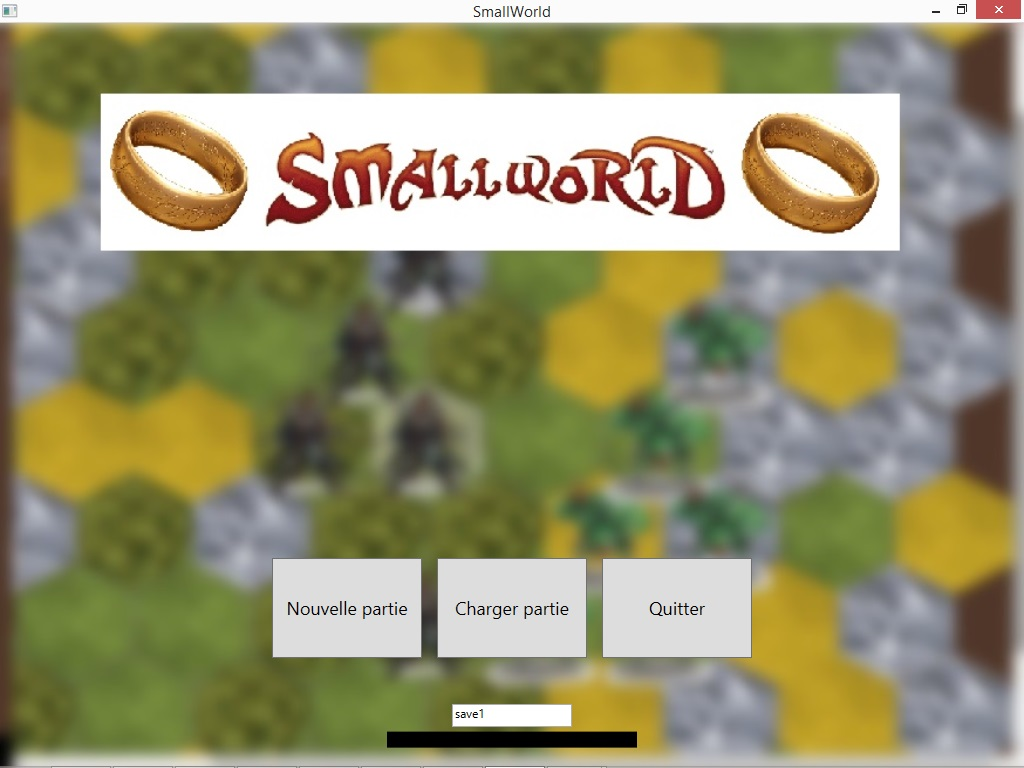
\includegraphics[scale=0.65]{img/init.jpg}
\caption{Fenêtre initiale}
\end{figure}
\newpage

\subsubsection{Fenêtre de création de partie}
Puis l'écran suivant s'affiche. Le premier joueur doit choisir son type de créature et rentrer son nom de joueur. Puis il valide. Après, c'est autour du second joueur, qui fera de même. Après avoir validé, la partie est lancée.

\begin{figure}[ht!]
\centering
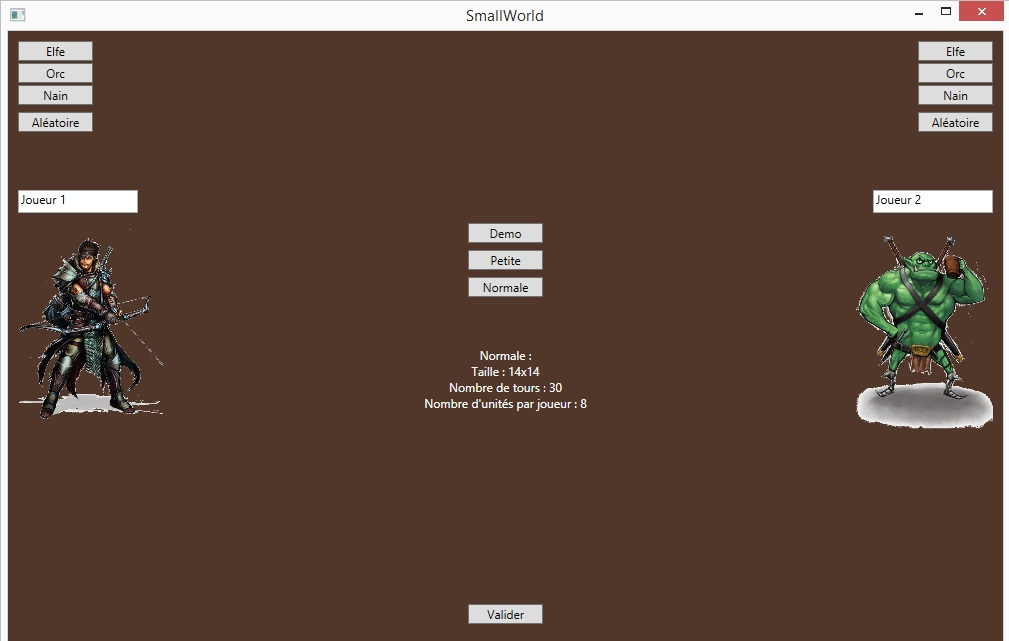
\includegraphics[scale=0.65]{img/crea.jpg}
\caption{Fenêtre de création de partie}
\end{figure}
\newpage


\subsubsection{Fenêtre de jeu}
Au cours de la partie, c'est la fenêtre suivante qui s'affiche. On remarque en haut à gauche que c'est au joueur 1 "Jean-Pierre" de jouer. Le nombre d'anneaux des deux joueurs est affiché au milieu.

\begin{figure}[ht!]
\centering
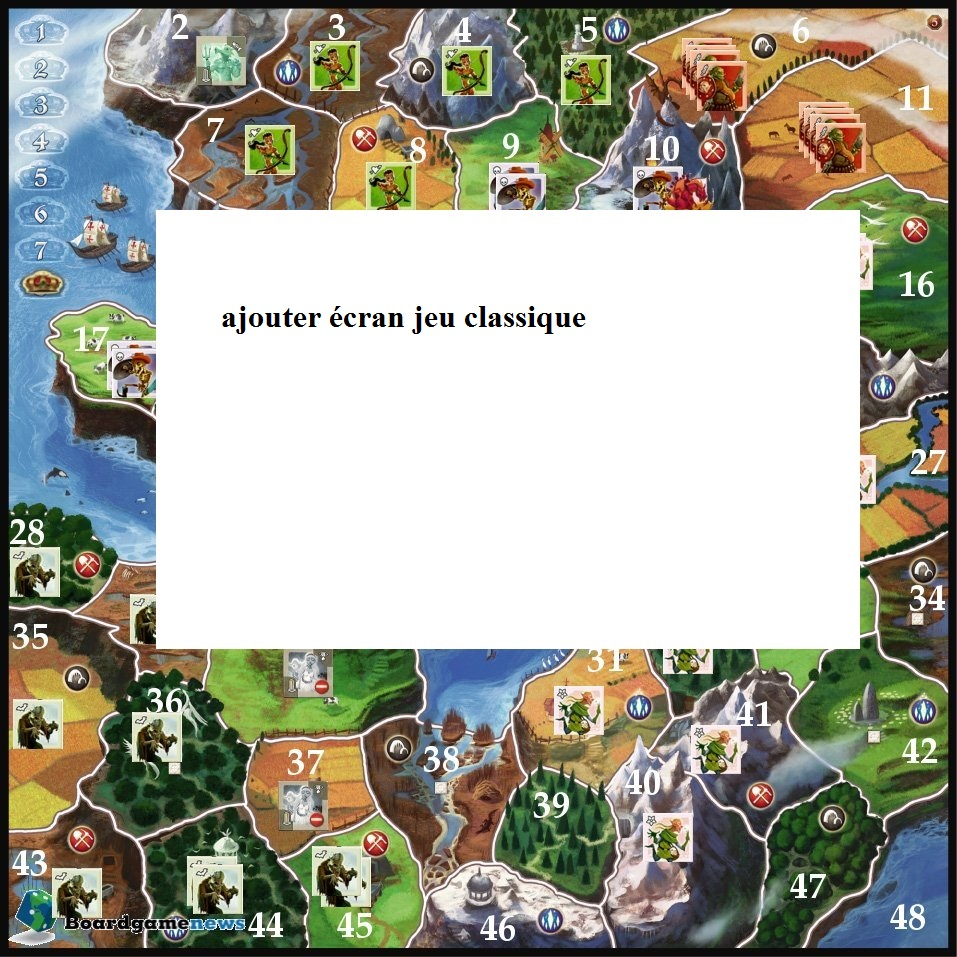
\includegraphics[scale=0.50]{img/jeu.jpg}
\caption{Fenêtre de jeu}
\end{figure}
\newpage

\subsection{Déroulement d'un tour}
\subsubsection{Généralités}

Les unités des joueurs sont placées automatiquement sur la carte, le joueur 1 toutes sur une case en haut à gauche, et le joueur 2 toutes sur une case en bas à droite. Il est décidé aléatoirement quel est le joueur qui commence la partie.
\newline
\newline
Les actions suivantes sont alors réalisées à chaque début de tour :
\begin{itemize}
\item Le nombre d'anneaux de contrôle est recalculé et affiché.
\item Le nombre de déplacement par unité est initialisé à 1.
\end{itemize}

\subsubsection{Actions du jeu}

Le joueur peut alors effectuer les actions suivantes :
\begin{itemize}
\item passer son tour
\item bouger une unité (ou plusieurs)
\item attaquer une unité sur une case
\item voir les caractéristiques d'une unité
\item utiliser l'algorithme de suggestion de mouvement
\newline
\end{itemize}

Il est possible de placer plusieurs unités sur la même case, mais il est déconseillé de le faire, car ils rapporteront moins d'anneaux actifs au décompte final.
\newline
\newline
Il n'est possible de bouger/attaquer que s'il reste assez de points de déplacement. Les coûts d'attaque et de déplacement peuvent varier selon les terrains et les unités.
\newline
En cliquant sur le bouton caractéristiques, il est possible de voir les caractéristiques de la pièce sélectionnée
\newline
\newline
L'algorithme de suggestion de mouvement suggère les meilleurs mouvements à faire pour une unité donnée. L'algorithme recherche les cases vides éloignées des unités alliées et des unités ennemies autant ou plus forte que l'unité courante. Il recherche le combat avec les unités plus faibles.
\newline
\newline

\newpage
\begin{figure}[ht!]
\centering
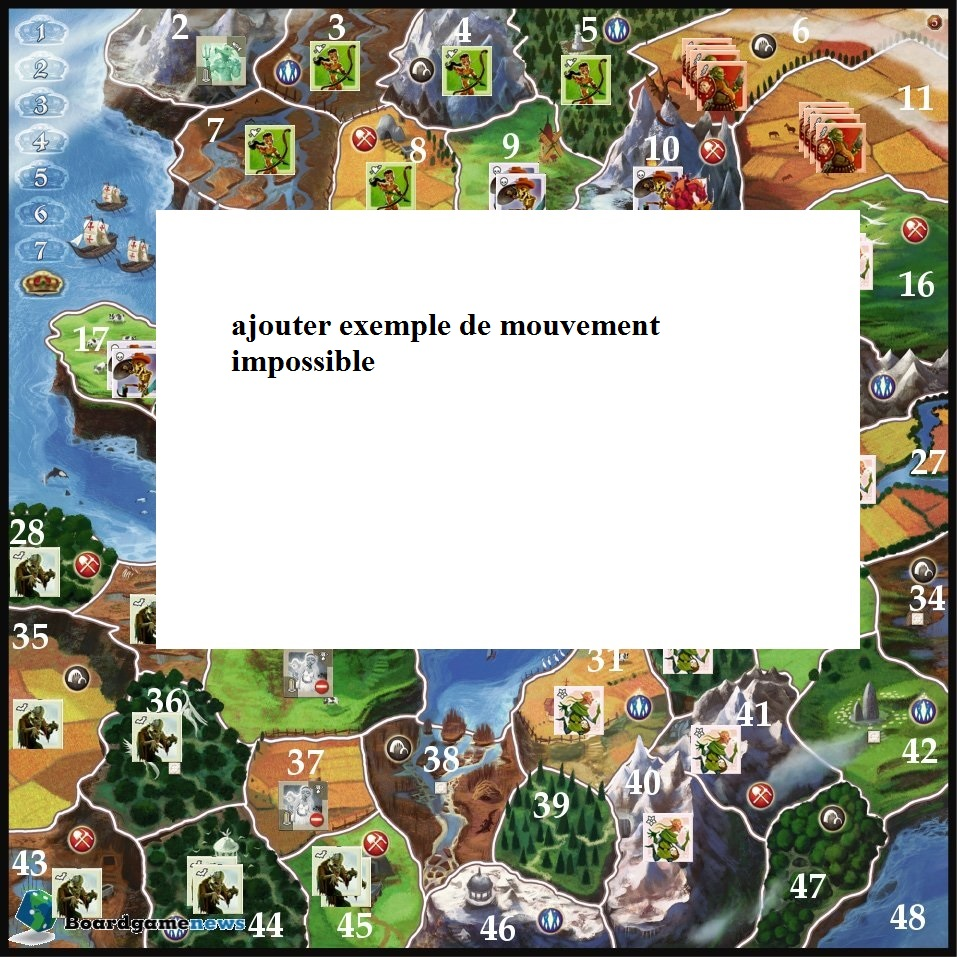
\includegraphics[scale=0.50]{img/exmovimp.jpg}
\caption{Exemple de mouvement impossible}
\end{figure}

\newpage
\begin{figure}[ht!]
\centering
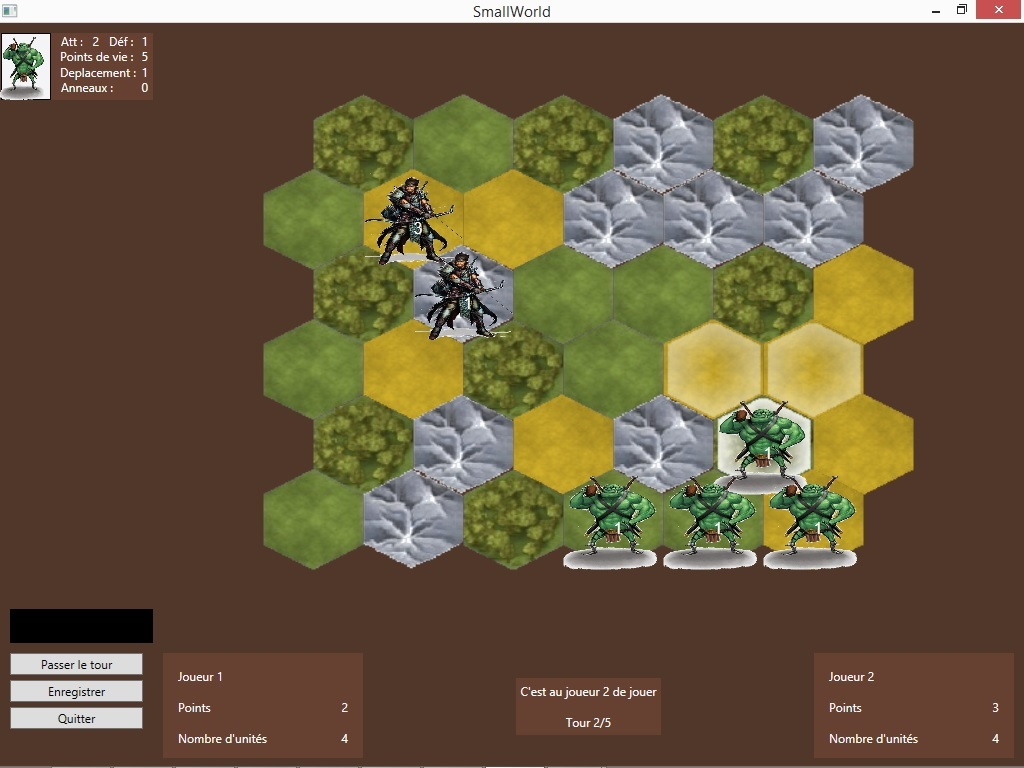
\includegraphics[scale=0.50]{img/algo.jpg}
\caption{Exemple applicatif de l'algorithme de suggestion}
\end{figure}

\newpage
\subsubsection{L'attaque}

Une attaque peut se solder par une victoire, une défaite, ou un match nul.
\newline
Pour chaque combat, un nombre d'attaque maximum est déterminé, entre 3 et le nombre de points de vie maximum des belligérants ajoutés à 2.
\newline
\newline
Les unités détiennent alors une probabilité d'attaquer, basé sur leurs attaques et défenses.
\newline
 L'attaquant est déterminé selon ces probabilités, et il inflige son attaque en blessures, pondéré par son nombre de points de vie.
\newline
Si aucune des unités ne meurt quand le nombre de combats maximum est atteint, il y a match nul.
\newline
\newline
Un message est affiché à la fin du combat.
\newline
 Les différents cas sont les suivants :
\begin{itemize}
\item En cas de victoire, l'unité prend la place de l'unité vaincue si la case est vide.
\item En cas de défaite, l'unité attaquante meurt.
\item En cas de match nul, l'unité attaquante se replie à sa place précédente.
\newline
\end{itemize}
Une attaque sur une case contenant plusieurs unités ennemies provoque le combat avec l'unité à plus forte défense, puis en cas de victoire, l'unité attaquera à nouveau les unités restantes de la case.

\begin{figure}[ht!]
\centering
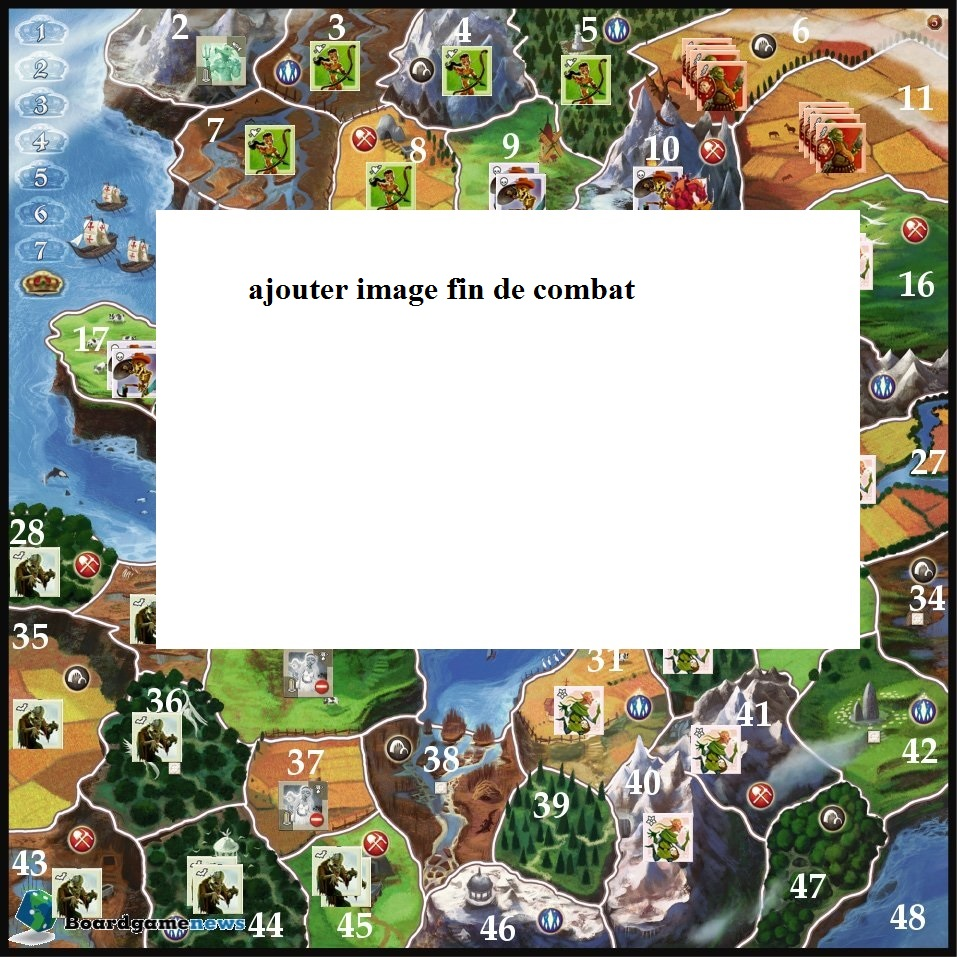
\includegraphics[scale=0.50]{img/fincombat.jpg}
\caption{Exemple de message de fin de combat}
\end{figure}

\newpage
\subsection{Fin de partie}

Au bout d'un certain nombre de tours, la partie prend fin. 
\newline
L'enchantement de Saruman fait effet et le joueur contrôlant le plus d'anneaux de contrôle retrouve l'anneau unique. 
\newline
\begin{center}
La partie est gagnée !
\end{center}
\begin{center}
En cas de match nul, les deux joueurs restent à égalité.
\end{center}